\hl{L1} Network refers to real systems; graph: a mathematical representation of a network, $G=(V,E)$. $e_{ij}\in E$ (directional) relationship between $v_i$ and $v_j$. 
\hlorange{Bipartite graph}$V=V_1 \cap V_2, v_i \in V_1, v_j \in V_2 \text{for all } e_{ij} \in E$.(user-item interactions recommender system).
\hlorange{Heterogeneous graph}$G=(V,E,R,T), r_{ij} \in R$ relation type, $T(v_i)$ node type
\hlorange{hypergraph} \( \mathcal{G} = (V, E, W) \), an edge \( e_j \) can connect any number of vertices, \( W_j \) denotes the weight of the hyperedge. 
\hlorange{dynamic graph} \( \mathcal{G}^t = (V^t, E^t) \), via sequentially updating \( \mathcal{G}^0 \) temporal events \( S = \{s_{t_1}, \dots, s_{t'}, \} \) happened before \( t \).  (transaction graph).
\hlorange{adjacent matrix, adjacency list} adjList[0] will have all the nodes which are connected (neighbour) to vertex 0 and so on. 
\hlorange{tasks} Node-level tasks tasks associated with individual nodes (traffic forecastting rs as v, connectivity as e). edge-level refer to tasks associated with a pair of nodes (Recommender sys). Graph-level tasks Infer if a molecular can be used as antibiotics. 
\hlorange{Unsupervised learning} aims to learn a mapping function without supervision signals to discover underlying patterns.
\hlorange{Semi-supervised learning} aims to learn an input-output mapping function based on partial supervision signals.


\hl{L2} \hlgreen{Traditional Graph Mining Approaches}: Step 1: Deign effective handcrafted features for node, link, graph level tasks by hand and prior.Step 2: Extract features and ML model training. 
\hlorange{Walk} is an alternating sequence of nodes and edges, starting with a node and ending with a node where each edge is incident with the nodes immediately preceding and following it.
\hlorange{Path} is a walk whose nodes are distinct. 
\hlorange{Connected component}. Given a graph \( \mathcal{G} = (V, E) \), a subgraph \( \mathcal{G}' = (V', E') \) is said to be a connected component if there is at least one path between any pair of nodes, and the nodes in \( V' \) are not adjacent to any vertices in \( V \setminus V' \).
\hlorange{Shortest path} \( p_{st\text{min}} = \arg\min |p| \) where \( p \) denotes the path with length \( |p| \). there could be more than one shortest path between any given pair of nodes.
\hlorange{Diameter} a connected graph \( \mathcal{G} = (V, E) \), \( \text{D}(\mathcal{G}) = \max_{v, w \in V} \min|p| \) max length of the shortest path
\hlorange{Complete graph} whose degree \( L = L_{\text{max}} \), and average degree is \( \langle k \rangle = N - 1 \).
    The maximum number of links a network of \( N \) nodes can have is:
    \( L_{\text{max}} = \binom{N}{2} = \frac{N(N - 1)}{2} \), average degree<k>=N-1
\hlorange{scale-free graph} most real-world graphs are sparse and follow power law distribution\({\mathbb  {P}}(d=k)\propto {\frac  {1}{k^{{\gamma }}}}\) \( \gamma \) is a parameter with \( 2 < \gamma < 3 \).
\hlgreen{Node level feature} node centrality Measure the importance of a node in a graph, ie, Node degree. \hlorange{Eigenvector centrality} the node’s centrality is proportional to the average centrality of its neighbors The eigenvector centrality can be rewritten as
\(c_v = \frac{1}{\lambda} \sum_{u \in N} A_{uv} c_u\)
\( c \) is the eigenvector and \( \lambda \) is the maximum eigenvalue. \( \lambda \mathbf{c} = A \mathbf{c} \) The centrality score is the eigenvector of \( A \). 
\hlblue{eg} The largest eigenvalue is 2.482 and its corresponding eigenvector is [1, 0.675, 0.675, 0.806, 1], where the degree of \(v_2, v_3, v_4\) are 2, but the eigenvector centrality of \(v_4\) is higher since it directly connected to \(v_1\) and \(v_5\), whose eigenvector centrality is higher.
 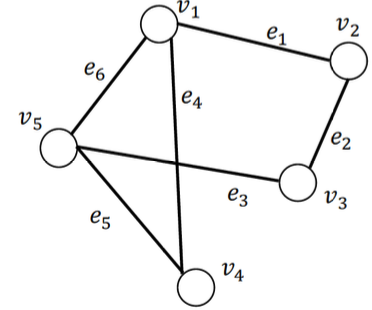
\includegraphics[height=0.025\textwidth]{figs/l2-4.png}
 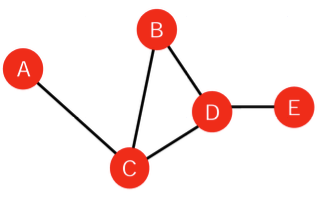
\includegraphics[height=0.025\textwidth]{figs/l2-5.png}
\hlorange{betweenness centrality} \(c(v) = \frac{\sum_{s,t \in V} \sigma_{st}(v)}{\sigma_{st}}\)
where \( \sigma_{st} \) denotes the total number of shortest paths from \( v_s \) to \( v_t \), and \( \sigma_{st}(v) \) indicates the number of these paths passing through \( v \). \hlblue{eg} \(c_A=c_B=c_E=0, c_C=c_D=3 (A-\underline{C}-B, A-\underline{C}-D, A-\underline{C}-D-E)\)
\hlorange{Clustering coefficient} The proportion of closed triangles in a node’s local neighborhood
\(c_u = \frac{\left| (v_1, v_2) \in E : v_1, v_2 \in N(u) \right|}{((d_u \times (d_u - 1) / 2 )} \)
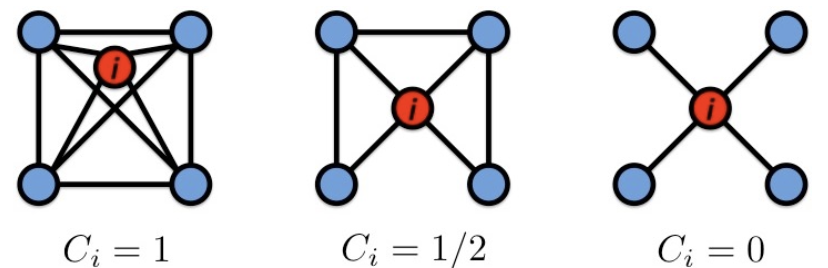
\includegraphics[height=0.025\textwidth]{figs/l2-1.png}
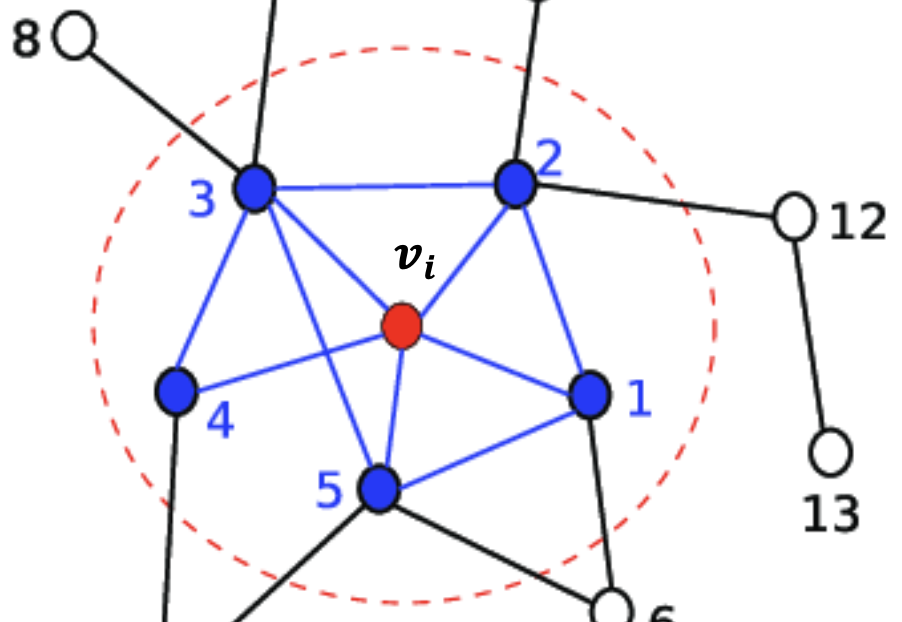
\includegraphics[height=0.025\textwidth]{figs/l2-2.jpg}
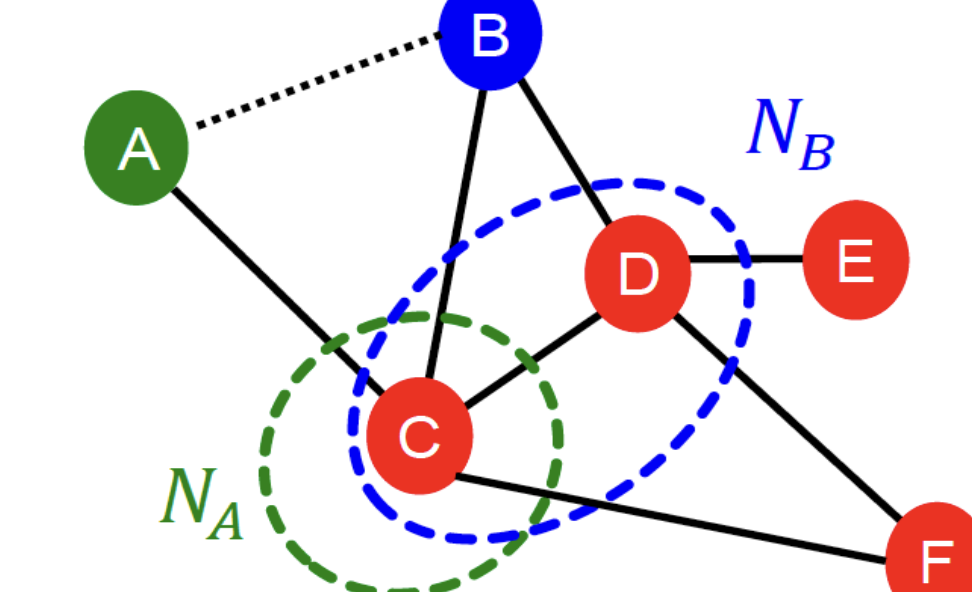
\includegraphics[height=0.025\textwidth]{figs/l2-3.png}
\hlorange{structure-based coefficient}Ego graph a subgraph that contains that node v, its neighbors, and all the edges between v and its neighborhood. 
\hlorange{Motifs and graphlets} Extends from triangles to more complex. \hlorange{limitation of node level feature} fail to encode the relationship between pair of nodes
\hlgreen{Link level feature: local neighbor overlap} \hlorange{shortest path distance} limitation: the topology between two nodes, overlap of neighbors, is overlooked.
\hlorange{Common neighbors:}\( S_c = |N(v_1) \cap N(v_2)| \)
\( S_c = 1 \)
\hlorange{Jaccard overlap:}
\(S_j = \frac{|N(v_1) \cap N(v_2)|}{|N(v_1) \cup N(v_2)|}\) 
\( S_j = \frac{1}{2} \)
\hlorange{Adamic-Adar index:}
\(S_AA = \sum_{v \in N(v_1) \cap N(v_2)} \frac{1}{\log(|N(v)|)}\) 
\( S_AA = \frac{1}{log4} \)
\hlgreen{global neighbor overlap}Limitation of local overlap: fail to handle node pairs without common neighbors.
\hlorange{Katz index}: count the number of paths of all lengths between a given pair of nodes \(S_katz=\sum_{i=1}^{\infty}\beta^i A^i[u,v]\), closed form \(S=(I-\beta A)^{-1} - I\), \(\beta\) discount factor, \(A^i[u,v]\) \# of walks length i between u and v.
\hlorange{Random walk feature} measure how likely we are to reach u from v via random walks.
\() S_{rw} = q_{u}[v] + q_{v}[u]\), \( q_{u} = (1 - c)(I - cP)^{-1} e_{u}\), \( e_{u} \) is the one-hot indicator vector for \( u \), \( P = AD^{-1} \) via personalized PageRank.
\( q_{u}[v]\) gives the stationary probability that random walk starting at node \( u \) visits node \( v \).
\hlgreen{graph kernel methods}
\hlorange{Weisfeiler-Lehman Kernel}
\hlorange{graph level featureLimitation}: overlook important global properties.
1. Assign initial label (color) \( l^0(v) \) to each node, e.g., based on node degree 
\( l^0(v) = d_v, \quad \forall v \in V \)
2. Iteratively update label by hashing current labels within the node’s neighborhood 
\( l^i(v) = \text{HASH}\left(\{ l^{i+1}(u) \, \forall u \in N(v) \}\right) \)
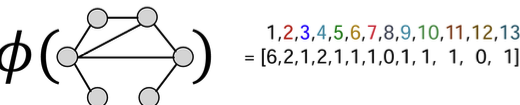
\includegraphics[height=0.025\textwidth]{figs/l2-8.png}
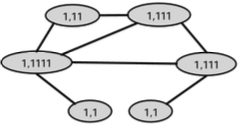
\includegraphics[height=0.02\textwidth]{figs/l2-6.png}
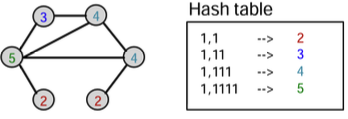
\includegraphics[height=0.025\textwidth]{figs/l2-7.png}
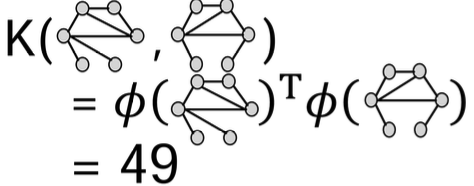
\includegraphics[height=0.025\textwidth]{figs/l2-9.png}
\hlorange{Graphlets Kernel} the distribution of small subgraph structures in the graph. but WL kernel is more efficient $O(\left|E\right|)$, and graphlet is $O(n^k)$ k is the size of graphlets.
\hlgreen{Spectral Graph Theory}
\hlorange{graph signal} \(u_i^TLu_i, u_i^TLu_0 = \lambda_0=0, u_i^TLu_1=\lambda_1, ...\)

